\chapter{PTC/FPP}
\label{c:ptc}
\index{PTC/FPP}
%----------------------------------------------------------------------------

The PTC/FPP library of \'Etienne
Forest handles Taylor maps to any arbitrary order. this is also known as Truncated Power
Series Algebra (TPSA). The core Differential Algebra (DA) package used by FPP was
developed by Martin Berz\cite{b:berz}.  

\begin{description}
\item[FPP] \Newline
The ``Fully Polymorphic Package'' (\vn{FPP}) library implements Differential Algebra (DA)
for the manipulation of Taylor maps. \vn{FPP} is purely mathematical in nature. It has no
knowledge of accelerators, magnetic fields, particle tracking etc.

\item[PTC] \Newline
The Polymorphic Tracking Code \vn{PTC} library is for accelerator simulation. It uses
\vn{FPP} as a back end for calculating such things as one turn maps.
\end{description}

PTC is used by \bmad when constructing Taylor maps and when the \vn{tracking_method}
\sref{s:tkm}) is set to \vn{symp_lie_ptc}.

For more information see the FPP/PTC manual\cite{b:ptc}.

%--------------------------------------------------------------------------
\section{Phase Space}
\label{s:ptc.space}
\index{PTC/FPP!phase space}

PTC uses different longitudinal phase space coordinates compared to \bmad.
\bmad's phase space coordinates are (\sref{s:phase.space})
\Begineq
  (x, p_x, y, p_y, z, p_z)
\Endeq
In PTC one can choose between several different coordinate systems. The one
that Bmad uses is 
\Begineq
  (x, p_x, y, p_y, p_t, c \Delta t)
\Endeq
where
\Begineq
  p_t = \frac{\Delta E}{P_0}
\Endeq
This choice of phase space is set in \Hyperref{r:set.ptc}{set_ptc}.  Specifically,
the PTC global variable \vn{DEFAULT}, which is of type
\vn{internal_states}, has the \vn{%time} switch set to \vn{True}.

\vn{vec_bmad_to_ptc} and \vn{vec_ptc_to_bmad} are conversion routines
that translate between the two. Actually there are a number of
conversion routines that translate between \bmad and PTC
structures. See \sref{r:ptc} for more details.

%--------------------------------------------------------------------------
\section{PTC Initialization}
\label{s:ptc.init}
\index{PTC/FPP!initialization}

One important parameter in PTC is the order of the Taylor maps.  By default \bmad will set
this to 3. The order can be set within a lattice file using the
\vn{parameter[taylor_order]} attribute.  In a program the order can be set using
\vn{set_ptc}. In fact \vn{set_ptc} must be called by a program before PTC can be used.
\vn{bmad_parser} will do this when reading in a lattice file.  That is, if a program does
not use \vn{bmad_parser} then to use PTC it must call \vn{set_ptc}. Note that resetting
PTC to a different order reinitializes PTC's internal memory so one must be careful if one
wants to change the order in mid program.

%--------------------------------------------------------------------------
\section{PTC Structures Compared to Bmad's}
\label{s:ptc.structures}

\bmad uses a \vn{lat_struct} structure to hold the information on a machine and a
\vn{lat_struct} has an array of \vn{branch_struct}s (the \vn{%branch(:)} component) with
each \vn{branch_struct} holding an array of \vn{ele_struct}s (the \vn{%ele(:)}
component). The \vn{ele_struct} holds the information on the individual elements. An
\vn{ele_struct} holds information about both the physical element and the reference orbit
through it.

PTC has a somewhat different philosophy as illustrated in \fig{f:ptc-struct}. A PTC
\vn{mad_universe} structure is very roughly equivalent to a \bmad \vn{lat_struct}. That
is, both structures can contain the description for an entire accelerator complex. Note
that it is standard in PTC to use two \vn{mad_universe} structures called \vn{m_u} and
\vn{m_t}. These two are defined globally. The difference between \vn{m_u} and \vn{m_t} is
that \vn{m_u} is used as a bookkeeping device for convenient accessing of all lattice
elements. On the other hand, \vn{m_t} contains the \vn{layouts} that can be used for
tracking.



equivalent to a \bmad \vn{branch_struct}. A
\vn{layout} has a pointer to a linked list of \vn{fibre} structures. Each \vn{fibre} has a
pointer to a \vn{magnet} structure which holds the information about the physical element
and each \vn{fibre} holds information about the reference orbit through the element.


With PTC, The top level structure \vn{mad_universe} has two components called \vn{%first}
and \vn{%last} which are pointers to the ends of an array of \vn{layout_array}
structures. Each \vn{layout_array} holds a \vn{layout} structure. A \vn{layout} structure
has pointers to the previous and next \vn{layout}s making a linked list of \vn{layout}s
indicated by the horizontal arrows. Each layout has pointers to a linked list of
\vn{fibre} structures. The \vn{fibre} structures represent the reference trajectory
through an element. Each \vn{fibre} structure has a pointer to a \vn{element} and an
\vn{elementp} structures which represent the physical element. With \bmad, the
\vn{lat_struct} roughly corresponds to the PTC \vn{layout_array(:)}, the
\vn{branch_struct} roughly corresponds to the PTC \vn{layout} and the \vn{element_struct}
roughly corresponds to the PTC \vn{fibre}, \vn{element} and \vn{elementp} structures.

%--------------------------------------------------------------------------

\begin{figure}[tb]
  \centering
  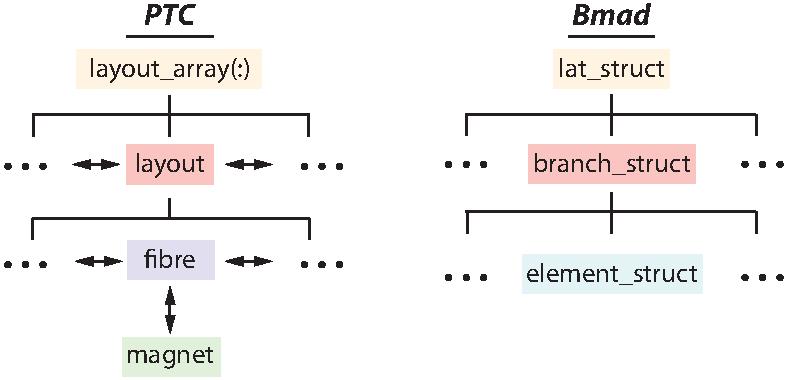
\includegraphics{ptc-structures.pdf}
  \caption[PTC structure relationships] { 
Simplified diagram showing the organization of the major PTC structures involved in
defining a lattice contrasted with \bmad.
  }
\label{f:ptc-struct}
\end{figure}

%--------------------------------------------------------------------------
\section{Variable Initialization and Finalization}
\label{s:ptc.var.init}
\index{PTC/FPP variable!initialization}

PTC variables must be initialized and finalized. This is done with
the\vn{alloc()} and \vn{kill()} routines. In addition, the \vn{real_8_init}
routine can initialize a \vn{real_8} array:
\begin{example}
  type (real_8) y8(6) 
  ...
  call real_8_init (y8)
  call kill (y8)
\end{example}

%--------------------------------------------------------------------------
\section{Correspondence Between Bmad Elements and PTC Fibres}.
\label{s:ele.fib}
\index{fibre}

When a PTC \vn{layout} is created from a \bmad \vn{lat_struct}
instance using the routine
\Hyperref{r:lat.to.ptc.layout}{lat_to_ptc_layout}, the correspondence
between the \bmad elements and the PTC fibres is maintained through
the \vn{ele%ptc_fibre} pointer. The following rules apply:
  \begin{enumerate}
  \item There will be marker \vn{fibre}s at the beginning and end 
of the \vn{layout}. The beginning \vn{fibre} will correspond to
\vn{branch%ele(0)}. The end \vn{fibre} will not have a corresponding
\bmad element.
  \item Generally there will be a one-to-one correspondence between
\vn{fibre}s and \vn{branch%ele} elements. The exception is where a
``hard edge'' model is used for tracking. In this case, there will be
three \vn{fibre}s for the \bmad element: Two drift \vn{fibre}s with a
\vn{fibre} of the appropriate type in between.  In this case,
\vn{ele%ptc_fibre} will point to the last (drift) \vn{fibre}.
  \end{enumerate}

Remember: The attributes like reference energy, etc. for a \bmad
\vn{ele_struct} instance are referenced to the exit end of the
element. For PTC the reference edge for a \vn{fibre} is the entrance
end.

%--------------------------------------------------------------------------
\section{Taylor Maps}
\label{s:ptc.taylor}
\index{PTC/FPP!Taylor Maps}

\index{PTC/FPP!real_8}\index{PTC/FPP!universal_taylor}
FPP stores its \vn{real_8} Taylor maps in such a way that it is not
easy to access them directly to look at the particular terms. To
simplify life, \'Etienne has implemented the
\vn{universal_taylor}structure:
\begin{example}
  type universal_taylor
    integer, pointer  :: n       ! Number of coefficients
    integer, pointer  :: nv      ! Number of variables
    real(dp), pointer :: c(:)    ! Coefficients C(N)
    integer, pointer  :: j(:,:)  ! Exponents of each coefficients J(N,NV)
  end type
\end{example}
\bmad always sets \vn{nv} = 6. \bmad overloads the equal sign to call 
routines to convert between \'Etienne's
\vn{real_8} Taylor maps and \vn{universal_taylor}:
\begin{example}
  type (real_8) tlr(6)           ! Taylor map
  type (universal_taylor) ut(6)  ! Taylor map
  ...
  tlr = ut                       ! Convert universal_taylor -> real_8
  ut = tlr                       ! Convert real_8 -> universal_taylor
\end{example}

%--------------------------------------------------------------------------
\section{Patches}
\label{s:ptc.patch}
\index{PTC/FPP!patch}

There is a significant difference between how patches are treated in
PTC and \bmad.  In PTC, a patch is just though of as a coordinate
transformation for propagating a particle from one \vn{fibre} to the
next. As such, the \vn{patch} is part of a \vn{fibre}. That is, any
\vn{fibre} representing tracking through quadrupoles, bends, etc. will
have patches for the entrance and exit ends of the \vn{fibre}.

With \bmad, on the other hand, a \vn{patch} is a ``first class''
element on par with all other elements be they quadrupoles, bends,
etc. When translating a \vn{patch} from \bmad to PTC, the \vn{patch}
is represented in PTC as a \vn{marker} element with a patch at the
exit end.

%--------------------------------------------------------------------------
\section{Number of Integration Steps \& Integration Order}
\label{s:ptc.step}

``Drift like'' elements in PTC will use, by default, only one
integration step. \bmad uses the default when translating from \bmad
lattice elements to PTC fibres. The \bmad lattice elements that are
drift like are:
\begin{example}
  drift
  ecollimator 
  instrument 
  monitor 
  pipe
  rcollimator 
\end{example}

When tracking, there is a trade-off between step size and integrator order. Higher order
means fewer steps are needed to get the same accuracy. But one higher order step is
computationally more intensive then one lower order step so what is the optimum order and
number of steps is dependent upon various factors like magnet strength and how fast the
field is varying. Generally, when the field is varying, such as in a wiggler, lower order
and more steps are favored. Also spin tracking is always 2nd order in PTC. So going to higher
order for the orbital tracking with less steps will cause the spin tracking to be less
accurate.

The way PTC ``resplitting'' routines work is that, for a given element, they start by
assuming that the tracking will be done using a 2\Nd order integrator, They then compute
the number of steps needed based upon the electric and magnetic field strengths. This
number is compared to a crossover limit point here named $C_1$. If the number of steps is
less than or equal to $C_1$ then the resplitting routine stops and tracking will
thereafter be done with a 2\Nd order integrator with the calculated number of steps. On
the other hand, if the number of steps is greater than $C_1$, the resplitting routine will
redo the calculation assuming 4\Th order integration. With 4\Th order integration, the
number of calculated steps will compared to a different crossover limit point here called
$C_2$. Again, if the number of steps is less than or equal to $C_2$, the routine will
assign 4\Th order tracking to the element. Otherwise, the routine will assign 6\Th order
tracking to the element with an appropriate number of steps.

The default crossover limit points are
\begin{align}
  [C_1, C_2] & = [30, 60] \qquad \text{For wiggler type elements.} \nonumber \\
  [C_1, C_2] & = [4, 18]  \qquad \text{For all other elements.} \nonumber 
\end{align}
The greater number for wigglers is a reflection of the fact that the wiggler field
is not constant.


%% PTC: defines real(8), real_8, probe, probe_8 
%% FPP: defines damap and c_damap and gmap
%% PTC only uses damap and c_damap for analysis not tracking.
